\subsection{Shadows}

In the Unity3D[ref] engine there are a number of way to light an environment, each way also has its own way of calculating shadows in the environment. Each way has its own disadvantages and advantages. Following will be experimentation and analysis of these lighting method will be carried out, to figure out which method is most useful for our use case. 


\begin{figure}
\centering
\begin{subfigure}[t]{0.33\textwidth}
\centering

\includegraphics[width=\linewidth]{figures/shadows/directional-cleaned}
\caption{directional}
\label{fig:directional}
\end{subfigure}%
    \hfill
\begin{subfigure}[t]{0.33\textwidth}
\centering
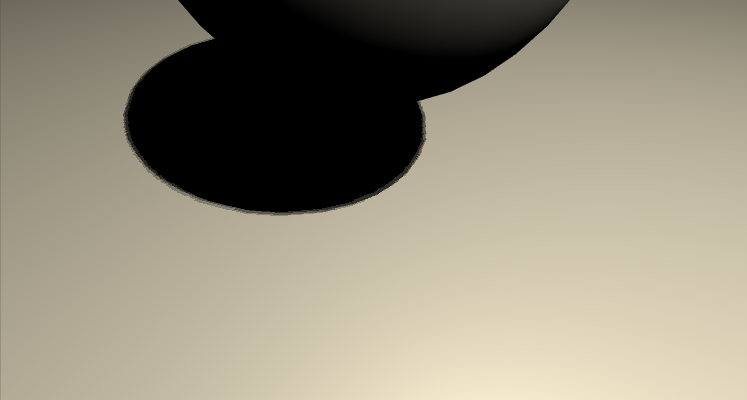
\includegraphics[width=\linewidth]{figures/shadows/point-cleaned}
\caption{point}
\label{fig:point}
\end{subfigure}%
    \hfill
\begin{subfigure}[t]{0.33\textwidth}
\centering

\includegraphics[width=\linewidth]{figures/shadows/point-far-cleaned}
\caption{point far}
\label{fig:point-far}
\end{subfigure}%

\caption{
(a) directional
(b) point
(c) point far
.}
\label{fig:rest-analysis}
\end{figure}


\begin{table}
  \centering
  \begin{tabular}{| c | c | c | c | }
    \hline
    & Narrow & Wide & Widest \\ \hline
    Close&  \begin{minipage}{.3\textwidth}
            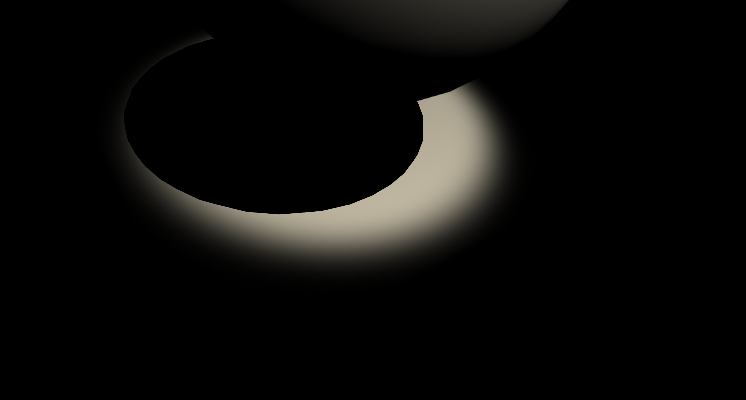
\includegraphics[width=\linewidth]{figures/shadows/spot-cleaned}
            \end{minipage}
            &
            \begin{minipage}{.3\textwidth}
            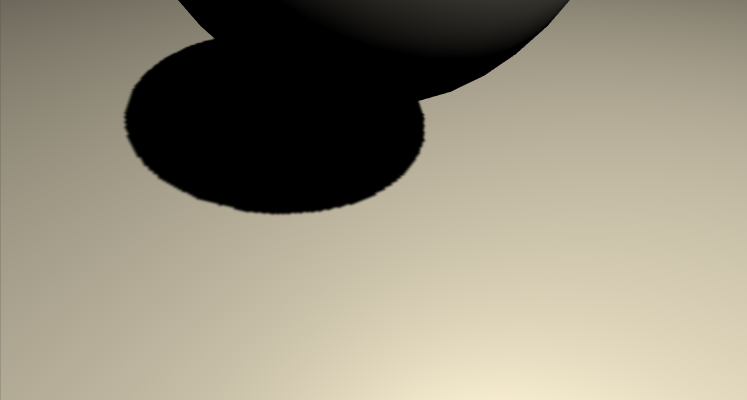
\includegraphics[width=\linewidth]{figures/shadows/spot-wide-cleaned}
            \end{minipage}
            & 
            \begin{minipage}{.3\textwidth}
            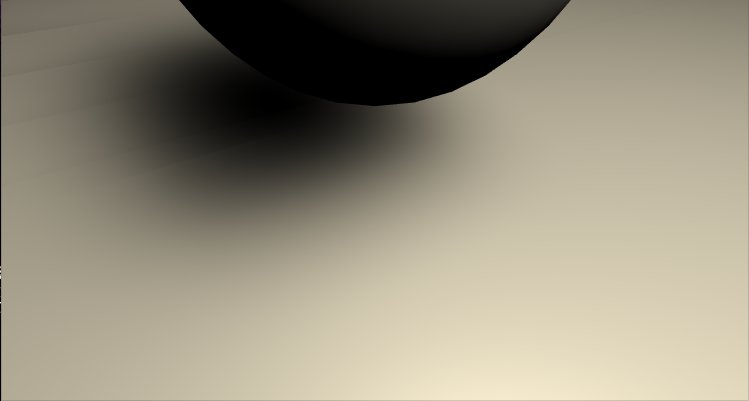
\includegraphics[width=\linewidth]{figures/shadows/spot-widest-cleaned}
            \end{minipage}
    \\ \hline
    Far &   \begin{minipage}{.3\textwidth}
            
\includegraphics[width=\linewidth]{figures/shadows/spot-far-cleaned}
            \end{minipage}
        &
            \begin{minipage}{.3\textwidth}
            
\includegraphics[width=\linewidth]{figures/shadows/spot-wide-far-cleaned}
            \end{minipage}
            & 
            \begin{minipage}{.3\textwidth}
            
\includegraphics[width=\linewidth]{figures/shadows/spot-widest-far-cleaned}
            \end{minipage}
    \\ \hline
  \end{tabular}
  \caption{Spot light analysis}\label{tbl:spot-analysis}
\end{table}